\documentclass[crop,tikz,pgf]{standalone}

\usetikzlibrary{arrows,automata}

\begin{document}
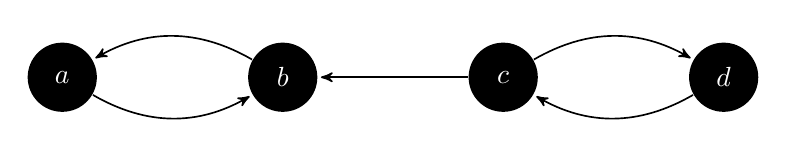
\begin{tikzpicture}[->,>=stealth',shorten >=1pt,auto,node distance=2.8cm,semithick]
	\tikzstyle{every state}=[fill=black,draw=none,text=white]

	\node[state] (B) {$b$};
	\node[state] (A) [left of=B] {$a$};
	\node[state] (C) [right of=B] {$c$};
	\node[state] (D) [right of=C] {$d$};

	\path (A) [bend right] edge (B);
        \path (B) [bend right] edge (A);
        \path (C) edge (B);
	\path (C) [bend left] edge (D);
	\path (D) [bend left] edge (C);
\end{tikzpicture}
\end{document}